\documentclass{article}

\usepackage{lipsum}        % lorem ipsum text
\usepackage{graphicx}      % include graphics
\usepackage{booktabs}      % nice tables
\usepackage{enumitem}      % lists


\title{My Paper}
\author{DKZ.2R}
\date{\today}

\usepackage[style=apa]{biblatex}
\addbibresource{sample-references.bib}

\usepackage{hyperref}

\usepackage{tikz}
\usetikzlibrary{shapes.geometric, arrows.meta, positioning}

% define styles
\tikzset{
	process/.style={
		rectangle,
		rounded corners,
		draw=black,
		fill=blue!20,
		text width=3cm,
		align=center,
		minimum height=1cm
	},
	file/.style={
		rectangle,
		draw=black,
		fill=orange!20,
		text width=3cm,
		align=center,
		minimum height=1cm
	},
	arrow/.style={
		->,
		>=Stealth,
		thick
	}
}


\hypersetup{
	colorlinks = true, 
	citecolor = blue,    % color for citations
	urlcolor = black,
}


\begin{document}

\pagenumbering{Roman} 

\maketitle

\newpage
\tableofcontents
\newpage
\listoftables
\newpage
\listoffigures
\newpage

\pagenumbering{arabic}

\section{Introduction}

\lipsum[1-2]


\section{Methods}

\lipsum[3]

\subsection{Figures with tikzpicture}


\begin{figure}[http]
	\centering
	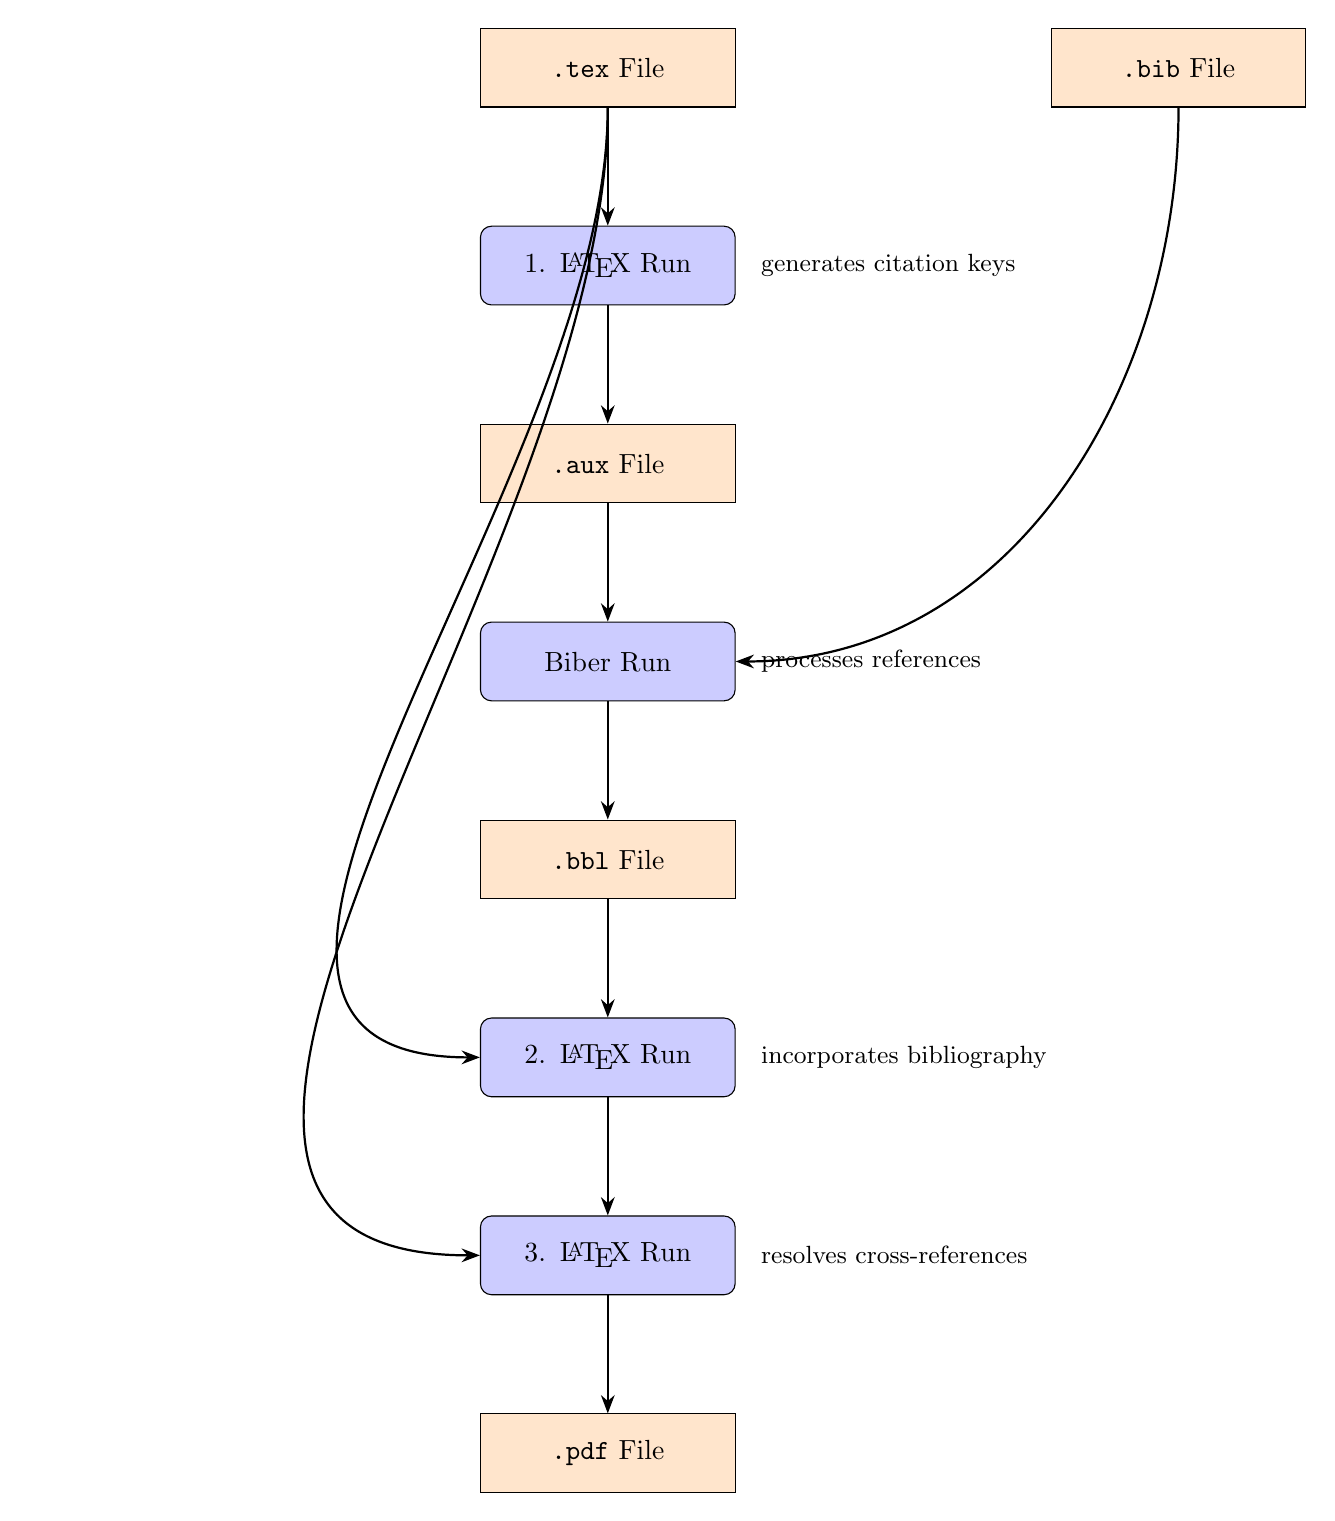
\begin{tikzpicture}[node distance=.25cm]
		
		% nodes
		\node (tex)     [file]                              {\texttt{.tex} File};
		\node (bib)     [file, right=4cm of tex]            {\texttt{.bib} File};
		\node (latex1)  [process, below=1.5cm of tex]       {1. \LaTeX\ Run};
		\node (aux)     [file, below=1.5cm of latex1]       {\texttt{.aux} File};
		\node (biber)   [process, below=1.5cm of aux]       {Biber Run};
		\node (bbl)     [file, below=1.5cm of biber]        {\texttt{.bbl} File};
		\node (latex2)  [process, below=1.5cm of bbl]       {2. \LaTeX\ Run};
		\node (latex3)  [process, below=1.5cm of latex2]    {3. \LaTeX\ Run};
		\node (pdf)     [file, below=1.5cm of latex3]       {\texttt{.pdf} File};
		
		% .tex feeds into all latex runs
		\draw [arrow] (tex) -- (latex1);
		\draw [arrow] (tex.south) to [out=270, in=180] (latex2.west);
		\draw [arrow] (tex.south) to [out=270, in=180] (latex3.west);
		
		% .bib feeds into biber
		\draw [arrow] (bib.south) to [out=270, in=0] (biber.east);
		
		% main flow
		\draw [arrow] (latex1) -- (aux);
		\draw [arrow] (aux)    -- (biber);
		\draw [arrow] (biber)  -- (bbl);
		\draw [arrow] (bbl)    -- (latex2);
		\draw [arrow] (latex2) -- (latex3);
		\draw [arrow] (latex3) -- (pdf);
		
		% annotations
		\node [right=0.2cm of latex1] {\small generates citation keys};
		\node [right=0.2cm of biber]  {\small processes references};
		\node [right=0.2cm of latex2] {\small incorporates bibliography};
		\node [right=0.2cm of latex3] {\small resolves cross-references};
		
	\end{tikzpicture}
	\caption{The LaTeX compilation process with citations using Biber}
	\label{fig:compilation}
\end{figure}


\subsection{Model}

\lipsum[10-11]

\subsection{Data Collection}

\lipsum[4]

\subsubsection{Unordered List}

The following items were collected:

\begin{itemize}
	\item First item
	\item Second item
	\item Third item
	\begin{itemize}
		\item Nested item 1
		\item Nested item 2
	\end{itemize}
	\item Fourth item
\end{itemize}

\subsubsection{Ordered List}

The data collection followed these steps:

\begin{enumerate}
	\item First step
	\item Second step
	\item Third step
	\begin{enumerate}
		\item Nested step 1
		\item Nested step 2
	\end{enumerate}
	\item Fourth step
\end{enumerate}


\subsection{Data Analysis}



\lipsum[5]

\section{Results}


\lipsum[6]

\subsection{Table Example}

\begin{table}[h]
	\centering
	\caption{Main table}
	\begin{tabular}{lcc}
		\toprule
		\textbf{Product} & \textbf{Value} & \textbf{Unit} \\
		\midrule
		Product A & 1.00 & kg \\
		Product B & 4.20 & kg \\
		Product C & 3.00 & kg \\
		\bottomrule
	\end{tabular}
	\label{tab:sample}
\end{table}

As shown in Table \ref{tab:sample}, the values increase linearly.

\subsection{Figure Example}

\begin{figure}[h]
	\centering
	% replace with your image
	
\includegraphics[width=0.5\textwidth]{my-awesome-image.png}
	\caption{Our main image.}
	\label{fig:sample}
\end{figure}

As shown in Figure \ref{fig:sample}, \lipsum[7]



\section{Conclusion}


\lipsum[10]	

The following conclusions can be drawn:

\begin{enumerate}
	\item Main conclusion
	\item Second conclusion
	\item Maybe we should not use list in the conclusion. 
\end{enumerate}

The importance of clear and effective communication in research cannot be
overstated. As noted by \textcite{Graham1995}, even everyday objects such
as the paperclip can serve as a metaphor for the complexity of modern
office life. This insight, combined with the statistical considerations
outlined by \textcite{Huff1954}, underlines the need for careful and
transparent reporting of results \autocite{Graham1995, Huff1954}.


\newpage

\printbibliography

\newpage 

\setcounter{page}{1}
\pagenumbering{roman}


\section{Appendix}

More information

\end{document}